%! Author = sosan
%! Date = 2025-03-24

% Preamble
\documentclass[a4paper,12pt]{article}

% Packages
\usepackage[utf8]{inputenc}
\usepackage[margin=1.75cm]{geometry}
\usepackage[T1]{fontenc}
\usepackage[french]{babel}
\usepackage{color}
\usepackage{hyperref}
\usepackage{graphicx}
\usepackage{booktabs}
\usepackage{hyperref}
\usepackage{amsmath}
\usepackage{amsfonts}
\usepackage{amssymb}
\usepackage{mathrsfs}
\usepackage{tikz}
\usepackage{multirow}
\usepackage{multicol}
\usepackage{csquotes}

% Document
\begin{document}

% Titre du document
\title{\textbf{Rapport Final : Classification des Tumeurs du Sein par Imagerie Ultrasonore \newline \large Une Approche Basée sur l'Intelligence Artificielle}}

\author{
    \small
    \begin{tabular}{ccc}
        \textbf{Sosane Mahamoud Houssein} & \textbf{Zeïnab Touré} & \textbf{Abidé Badjoudoum} \\
        HOUS92310307 & TOUZ63280208 & BADA09349800 \\
        \textit{hous44@uqo.ca} & \textit{touz08@uqo.ca} & \textit{bada20@uqo.ca} \\
    \end{tabular}
}

\normalsize
\date{}
\maketitle



\begin{abstract}
Ce projet vise à développer un système de classification des tumeurs du sein en utilisant des images ultrasonores et des techniques d'apprentissage profond. Le système prend en entrée des images échographiques et produit en sortie une classification bénigne, maligne ou normale. Nous avons utilisé un modèle ResNet-18 pré-entraîné et l'avons affiné sur un ensemble de données annotées. Les résultats montrent une précision élevée, démontrant l'efficacité de notre approche.
\end{abstract}

\section{Définition de la Tâche}

\subsection{Description de la Tâche}
Le cancer du sein est la cause de mort la plus fréquente chez les femmes dans presque chaque pays \cite{sancho2019epidemiologie}. On estime qu'un million de femmes chaque année sont diagnostiquées avec le cancer du sein et plus de 410 000 sont à risque de mourir de cette maladie \cite{frikha2021aperccu}. Toutefois, une détection rapide de la tumeur permettra de réduire le taux de mortalité. Cette tumeur prend naissance dans les cellules du sein et peut être classifié comme bénigne ou maligne.

La masse mammaire est le signe le plus évident du cancer du sein. De nombreuses techniques d'imageries sont utilisés dans le domaine médicale pour assurer le dépistage précoce de la tumeur, tels que: l'échographie mammaire (ultrasons), la mammographie et l'IRM mammaire \cite{soltani2025detection}.

Notre projet intègre des approches d'apprentissage automatique et profond dans les systèmes d'aide au diagnostic. L'objectif principal de cette approche est de concevoir un système capable de détecter les tumeurs puis de les classifier.

Notre système prend en entrée des images échographiques de tumeurs du sein et les classe en trois catégories : bénignes, malignes ou normales. La sortie est une étiquette de classe accompagnée d'un score de confiance.

\subsection{Délimitation}
La tâche se limite à la classification des images ultrasonores (échographie mammaire) et n'inclut pas d'autres modalités d'imagerie (comme la mammographie). Elle se concentre sur trois classes principales, ce qui la rend gérable tout en restant cliniquement pertinente.

\subsection{Pertinence IA}
L'IA est particulièrement adaptée à cette tâche en raison de sa capacité à extraire des caractéristiques complexes des images et à généraliser à partir de grandes quantités de données. Les méthodes d'apprentissage profond, comme les réseaux de neurones convolutifs, ont montré des performances supérieures dans les tâches de classification d'images médicales \cite{mayouf2021preparation}.

\section{Brève Revue de la Littérature}

Plusieurs études ont exploré l'utilisation de l'IA pour la classification des tumeurs du sein. Par exemple, les travaux venant du laboratoire Hubert Curien de Saint-Etienne\cite{mayouf2021preparation} et l'université De Echahid Echeikh Larbi Tébessi-Tébessa \cite{soltani2025detection} ont utilisés des réseaux de neurones convolutifs pour distinguer les tumeurs bénignes des malignes avec de très hauts taux de précisions. Notre approche diffère par l'utilisation de ResNet-18 et par l'inclusion d'une classe "normale" pour améliorer la spécificité.

\section{Matériel et Méthodes}

\subsection{Infrastructure}
Nous avons utilisé Python avec les bibliothèques PyTorch pour l'apprentissage profond, OpenCV pour le prétraitement des images et Sklearn, principalement pour la séparation des données et l'évaluation du modèle de classification.

\subsection{Méthodes}
\subsubsection{Ensemble de Données}
Nous avons utilisé le Dataset\_BUSI\_with\_GT \cite{al2020dataset} sur la plateforme Kaggle, qui contient des images échographiques annotées collectés dans l'hôpital Baheya. Les images sont en noir et blanc de dimensions diverses. Cette diversité au niveau des dimensions des images de la base de données est expliqué par le fait que les spécialistes de l'hôpital Baheya ont recadré les images pour supprimer les limites sans importances des images \cite{al2020dataset}. La diversité des dimensions des images a été décrie dans le \autoref{tab:dimensions}.

La classe \enquote{UltrasoundDataset} a été créée afin de gérer le chargement des données:
\begin{verbatim}
# Chargement des données d'entraînement
training_dataset = UltrasoundDataset(
    X_train,
    masked_train,
    y_train,
    transform =
        ImageTransform(
            image_training_transform,
            masked_transform
        ))
\end{verbatim}

Les images de la base de données sont classifiées dans les catégories suivantes: bégnines, malignes et normales. Il y a 780 images ultrasonores dans la base de données et sont réparties de cette maniére:
\begin{itemize}
    \item Bénignes : 437 images (56\%)
    \item Malignes : 210 images (27\%)
    \item Normales : 133 images (17\%)
\end{itemize}

\begin{table}[h]
    \centering
    \caption{Statistiques des dimensions d'images}
    \begin{tabular}{lcc}
        \toprule
        & Hauteur (px) & Largeur (px) \\
        \midrule
        Minimum & 310 & 190 \\
        Maximum & 719 & 1048 \\
        \bottomrule
    \end{tabular}
    \label{tab:dimensions}
\end{table}

Des spécialistes de l'hôpital de Baheya ont analysés chaque image, puis ont créées une version masqué pour chaque image prise par l'échographie. Dans la base de données, les images masqués finissent avec le suffixe \enquote{\_mask}. Ces images masqués délimitent en blanc la tumeur sur les échographies. Naturellement, les images venant d'une patiente sans tumeur (classifié comme normale) sont entièrement absent de pixels blancs. Un exemple d'images venant des échographies et de leurs masques correspondants peut être trouvé dans la \autoref{fig:samples}.

\begin{figure}[h]
    \centering
    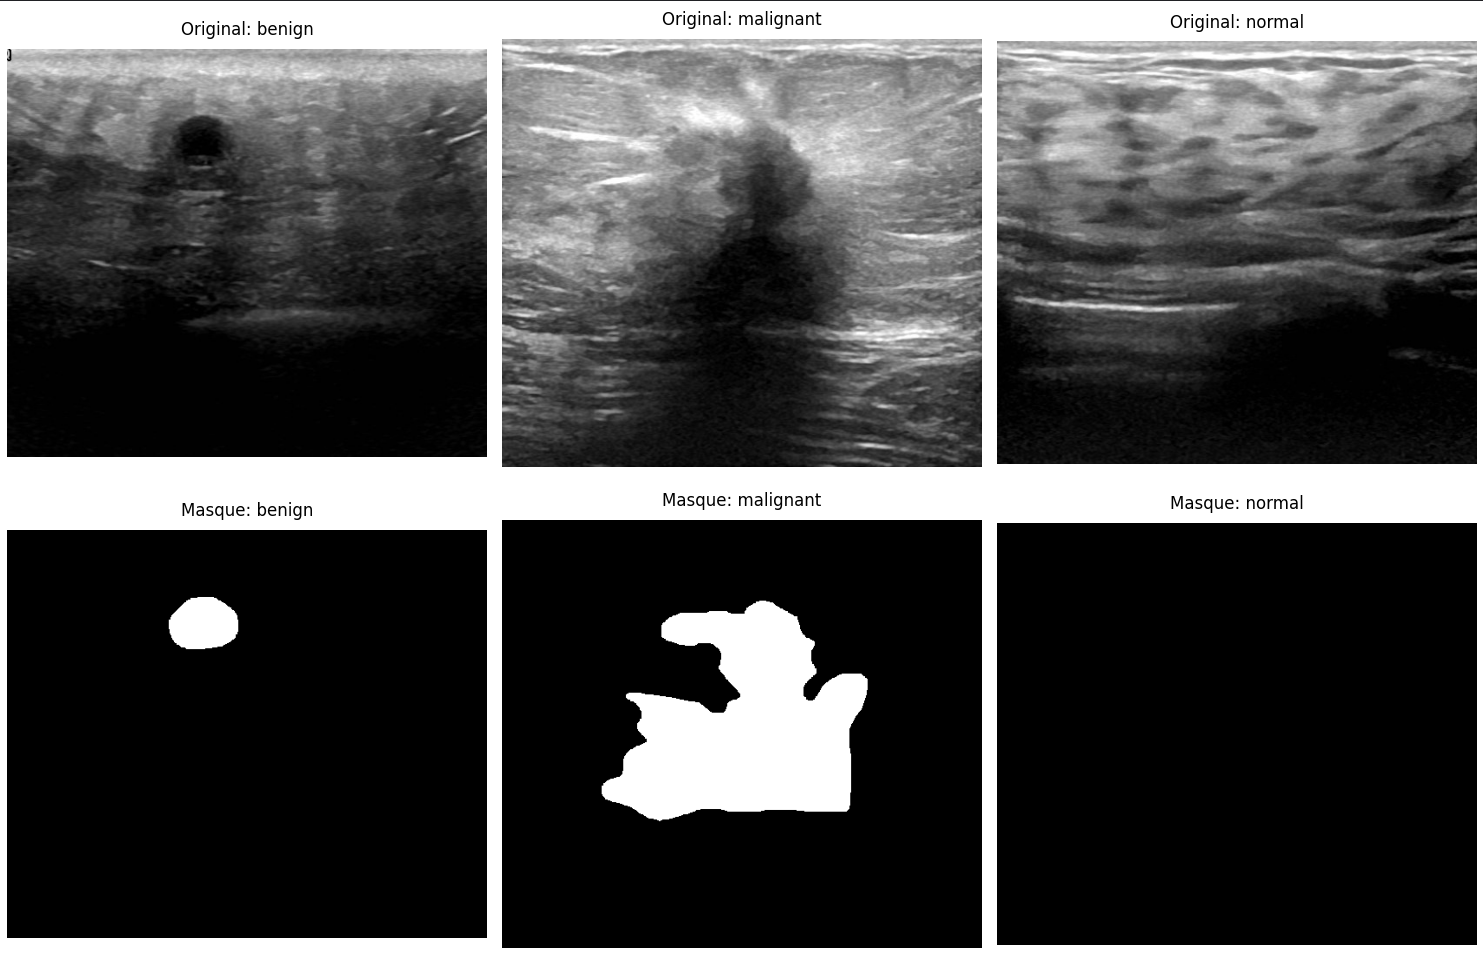
\includegraphics[width=0.8\textwidth]{sample_images.png}
    \caption{Exemples d'images avec leurs masques correspondants}
    \label{fig:samples}
\end{figure}

Une analyse supplémentaire des images masquées a été performé afin de connaître certaines statisques clés de la superficie tumorale (en pixels), les résultats de cette analyse est inclues dans le \autoref{tab:masks}.

\begin{table}[h]
    \centering
    \caption{Superficie tumorale moyenne (en pixels)}
    \begin{tabular}{lcccc}
        \toprule
        Classe & Moyenne & Médiane & Min & Max \\
        \midrule
        Bénin & 20,734 & 10,263 & 804 & 209,121 \\
        Malin & 43,376 & 34,433 & 569 & 167,411 \\
        Normal & 0 & 0 & 0 & 0 \\
        \bottomrule
    \end{tabular}
    \label{tab:masks}
\end{table}

Les données ont été divisées en ensembles d'entraînement (80\%) et de test (20\%).

Afin de rendre la base de données utiles pour la création du modèle d'apprentissage profond, certaines tâches doivent être complétés.

La phase de prétraitement et de transformation des données prends en compte les analyses d'exploration de la base de données. Il y a premièrement un probléme de déséquilibre des classes, car la majorité des images proviennent de patientes atteintes de tumeur bégnine (soit 56\% des données). Pour prévenir la possibilité que le modèle soit biaisé par les images classifiées comme \enquote{bégnines}, il est impératif d'implémenter une fonction de coût pondérée:

\begin{equation}
        w_c = \frac{N}{C \times N_c}
    \end{equation}
où $N$=total, $C$=classes, $N_c$=échantillons par classe

De plus, l'analyse préliminaire a aussi détecté la très grande grande variété de dimensions des images. Les images ont alors été redimensionnées à $256\times256$ px en préservant le ratio d'aspect. Les images originales ont aussi reçues ces transformations supplémentaires:

\begin{itemize}
        \item Rotation aléatoire ($\pm15^\circ$)
        \item Retournement horizontal
        \item Ajustement de contraste
\end{itemize}

Les images originales ont été normalisés avec les statistiques calculés par la base de données d'ImageNet, soit: $\mu=[0.485,0.456,0.406]$, $\sigma=[0.229,0.224,0.225]$

Quant aux images masqués, elles ont simplement été redimensionnées et recadrées.

Une classe appelé \enquote{ImageTransform} a été créée pour simplifier le processus de prétraitement des données.

\begin{verbatim}
# Classe pour prétraiter et transformer les données
class ImageTransform:
    def __init__(self, image_transform, masked_transform):
        self.image_transform = image_transform
        self.masked_transform = masked_transform

    # Transformer les images et masques
    def __call__(self, image, mask):
        return self.image_transform(image), self.masked_transform(mask)
)
\end{verbatim}

\subsubsection{Modèle}
Nous avons utilisé ResNet-18 pré-entraîné sur ImageNet et l'avons affiné avec nos données. La fonction de perte utilisée est l'entropie croisée, et l'optimiseur est Adam.

\enquote{BreastUltrasoundModel} est la classe de l'architecture du modèle de réseaux de neurones. La classe prend en compte les caractéristiques des images originales, leurs masques correspondants et la superficie des tumeurs.

\begin{verbatim}
# Configuration initiale de l'entraînement du modèle avec la classe BreastUltrasoundModel
model = BreastUltrasoundModel().to(device)
criterion = nn.CrossEntropyLoss(weight=categorie_weights.to(device))
optimizer = optim.Adam(model.parameters(), lr=0.001, weight_decay=1e-4)
scheduler = optim.lr_scheduler.ReduceLROnPlateau(optimizer, 'min', patience=3)
early_stopping = EarlyStopping(patience=5)
)
\end{verbatim}

La taille des batchs est de 32 échantillons à la fois, pour les données d'entraînement et de validation.

La boucle d'entraînement dure environ 9 epochs (\textit{époques} en français), soit 9 itérations de la boucle d'entraînement.

\subsection{Évaluation}
Les performances ont été évaluées en termes de précision, rappel et F1-score. Nous avons également utilisé des matrices de confusion pour analyser les erreurs de classification. La \autoref{fig:confusionmatrix} contient la matrice de confusion de l'epoch 20 lors de l'entraînement.

Une courbe ROC a aussi été générée pour mesurer la performance du classificateur. La courbe ROC donne le taux de vrais positifs en fonction du taux de faux positifs \cite{frwiki:224482682}.

\section{Résultats}

\subsection{Présentation des Résultats}
\begin{table}[h]
\centering
\caption{Métriques de performance}
\begin{tabular}{lccc}
\toprule
Classe & Précision & Rappel & F1-score \\
\midrule
Bénigne & 0.84 & 0.83 & 0.83 \\
Maligne & 0.65 & 0.67 & 0.66 \\
Normale & 1.00 & 1.00 & 1.00 \\
\bottomrule
\end{tabular}
\end{table}

\begin{figure}[h]
\centering
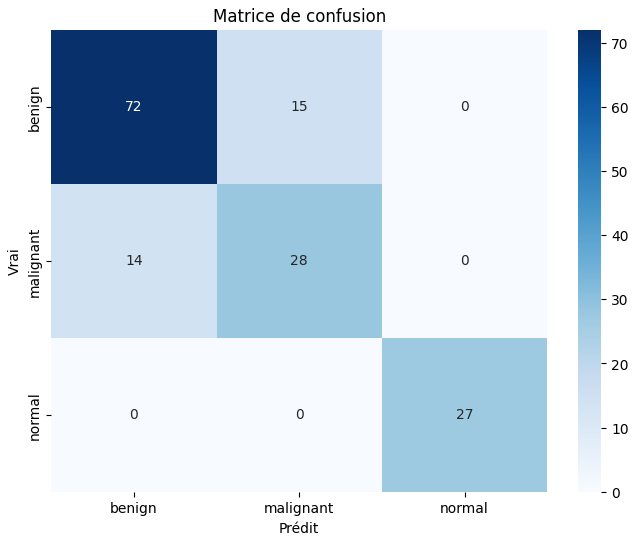
\includegraphics[width=0.7\textwidth]{confusion_matrix.png}
\caption{Matrice de confusion}
\label{fig:confusionmatrix}
\end{figure}

Nous avons d'autant plus performé une évaluation du modèle avancé en générant une courbe ROC. La courbe ROC représente une courbe de probabilité \cite{narkhede2018understanding}.
Le score AUC (\enquote{\textit{Area Under Curve}}, soit l'aire sous la courbe), va quant à elle, représente le degrée de séparabilité. Il permet de déterminer à quel point un modèle est capable de distinguer les classes \cite{narkhede2018understanding}. La \autoref{fig:curve} représente la courbe ROC.
\clearpage

\begin{figure}[h]
\centering
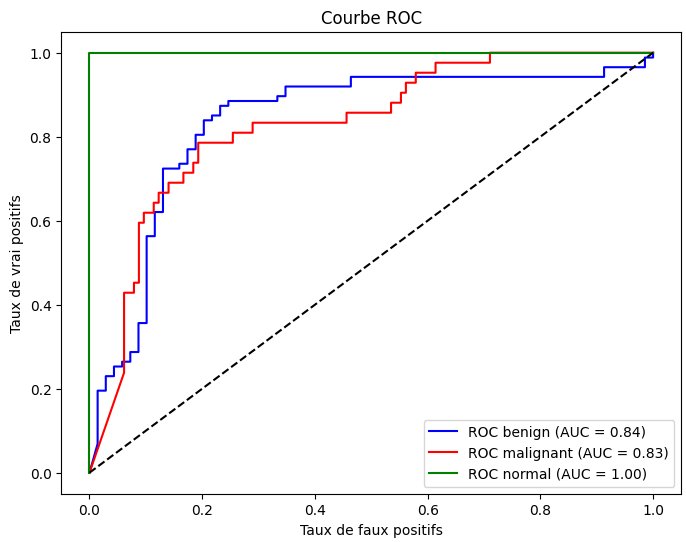
\includegraphics[width=0.7\textwidth]{roc_curve.png}
\caption{Courbes ROC générées pour le classificateur BreastUltrasoundModel}
\label{fig:curve}
\end{figure}

\clearpage
\begin{figure}[h]
\centering
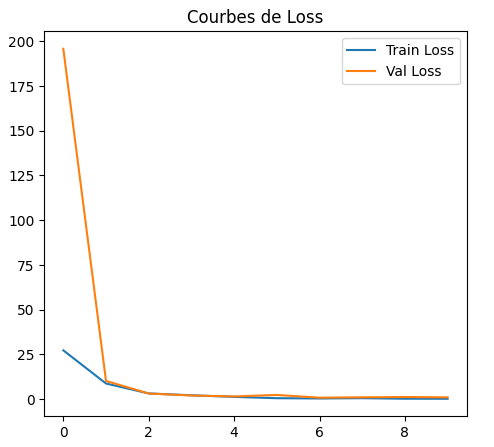
\includegraphics[width=0.5\textwidth]{loss_curve.png}
\caption{Courbes de perte (\textit{Loss}) générées pour le classificateur BreastUltrasoundModel}
\label{fig:losscurve}
\end{figure}

\begin{figure}[h]
\centering
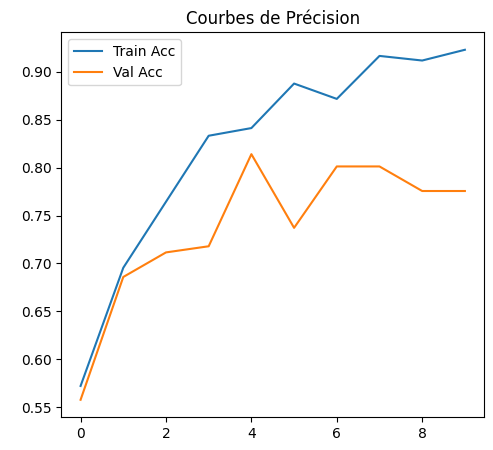
\includegraphics[width=0.5\textwidth]{accuracy_curve.png}
\caption{Courbes de précision (\textit{Accuracy}) générées pour le classificateur BreastUltrasoundModel}
\label{fig:accuracycurve}
\end{figure}


\subsection{Analyse}
Le modèle a montré une bonne performance globale, avec un F1-score moyen de 0.83. Le modèle excellait particulièrement avec la classification des images normales. Les erreurs de classification étaient principalement entre les classes bénignes et malignes, ce qui est cohérent avec la littérature.

De plus, chaque catégorie du classificateur a obtenu un haut score AUC. Le \autoref{tab:auccurve} représente le score AUC pour chaque classe.

\begin{table}[h]
\centering
\caption{Score AUC pour chaque classe}
\begin{tabular}{lccc}
\toprule
Classe & Score AUC \\
\midrule
Bénigne & 0.84 \\
Maligne & 0.83 \\
Normale & 1.00 \\
\bottomrule
\end{tabular}
\label{tab:auccurve}
\end{table}

\section{Conclusion}

\subsection{Résumé des Résultats}
Notre système a atteint une précision élevée dans la classification des tumeurs du sein, démontrant la faisabilité d'utiliser ResNet-18 pour cette tâche.

\subsection{Perspectives}
Pour améliorer le système, nous envisageons d'incorporer des données multimodales et d'explorer des architectures plus récentes comme Vision Transformers. Une validation externe sur des données indépendantes serait également bénéfique.

\clearpage
\bibliographystyle{plain}
\bibliography{references}


\end{document}